\documentclass[12pt]{beamer}

\usepackage[utf8]{inputenc}
\usepackage{fontspec}


%\usepackage[brazil]{babel} % formatação brasileira e traduções

\def\style{light}% escolha light (claro) ou dark (escuro) / choose either light or dark

% cores utilizadas nas logos / colors used in the logo
\definecolor{UnBgray}{rgb}{0.13671875, 0.12109375, 0.125}
\definecolor{UnBgreen}{rgb}{0.0, 0.545098, 0.26171875}
\definecolor{UnBblue}{rgb}{0.0, 0.2578125, 0.48828125}

\setmainfont{./UnB-Office_Regular.ttf} % fontes oficiais / official fonts

\def\dark{dark}

\ifx \style \dark
% definições do tema escuro / dark theme definitions
\logo{
\includegraphics[width=1.5cm]{logo_unb_dark.PNG}}

\setbeamercolor{frametitle}{fg=UnBgreen}
\setbeamercolor{normal text}{fg=white}
\setbeamercolor{background canvas}{bg=UnBgray}
\setbeamercolor{title}{fg=UnBgreen}
\setbeamercolor{structure}{fg=UnBgreen} % itemize, enumerate, etc

\else
% definições do tema claro / light theme definitions
\logo{
\includegraphics[width=1.5cm]{logo_unb_light.PNG}}

\setbeamercolor{background canvas}{bg=black}
\setbeamercolor{frametitle}{fg=UnBblue}
\setbeamercolor{normal text}{fg=black}
\setbeamercolor{background canvas}{bg=white}
\setbeamercolor{title}{fg=UnBblue}
\setbeamercolor{structure}{fg=UnBblue} % itemize, enumerate, etc

\fi

\let\oldfootnote\footnote
\renewcommand\footnote[1][]{\oldfootnote[frame,#1]}

\title{ns-3 with CMake}
\author{Gabriel Ferreira}
\date{\today}
\institute{University of Brasília}


\begin{document}
\maketitle

\begin{frame}{My goals with CMake}
    
    IDE support
    \begin{enumerate}
        \item Easier debugging and profiling
        \item Auto-completion
        \item Macro expansion (showing what the actual code looks like)
        \item Visually show errors, warnings, unused includes, etc
    \end{enumerate}
\end{frame}

\begin{frame}{Unsupported/incomplete features}
    \begin{enumerate}
        \item Bake integration
        \item NSC examples
        \item Planetlab examples
        \item Python bindings 
        \item[] \hspace{1em}{\footnotesize The code is there, but apiscan and generation fail for some modules}
    \end{enumerate}
\end{frame}

\begin{frame}{What is missing?}
    \begin{enumerate}
        \item Implement remaining features
        \item[] \hspace{1em} {\footnotesize I can do that!}
        \item Stylistic and workflow related refactoring
        \item[] \hspace{1em} {\footnotesize I need maintainers feedback}
        \item Update ns-3 official docs with instructions
    \end{enumerate}
\end{frame}   

\begin{frame}{Current workflow}
    \begin{enumerate}
        \item Create a new module
        \item Configure CMake
        \item Call the generated build system to build (e.g. ninja)
        \item Call binaries directly or via the IDE
        \item Debug via the IDE
    \end{enumerate}
\end{frame} 

\begin{frame}{Current workflow}{Create a new module}
    \begin{enumerate}
        \item Create a new folder with a CMakeLists.txt file. Set library name, list of source files and add the macro at the end.
    \end{enumerate}
    
    
    \begin{figure}[h]
        \vspace{-1em}
        \hspace{-16em}
        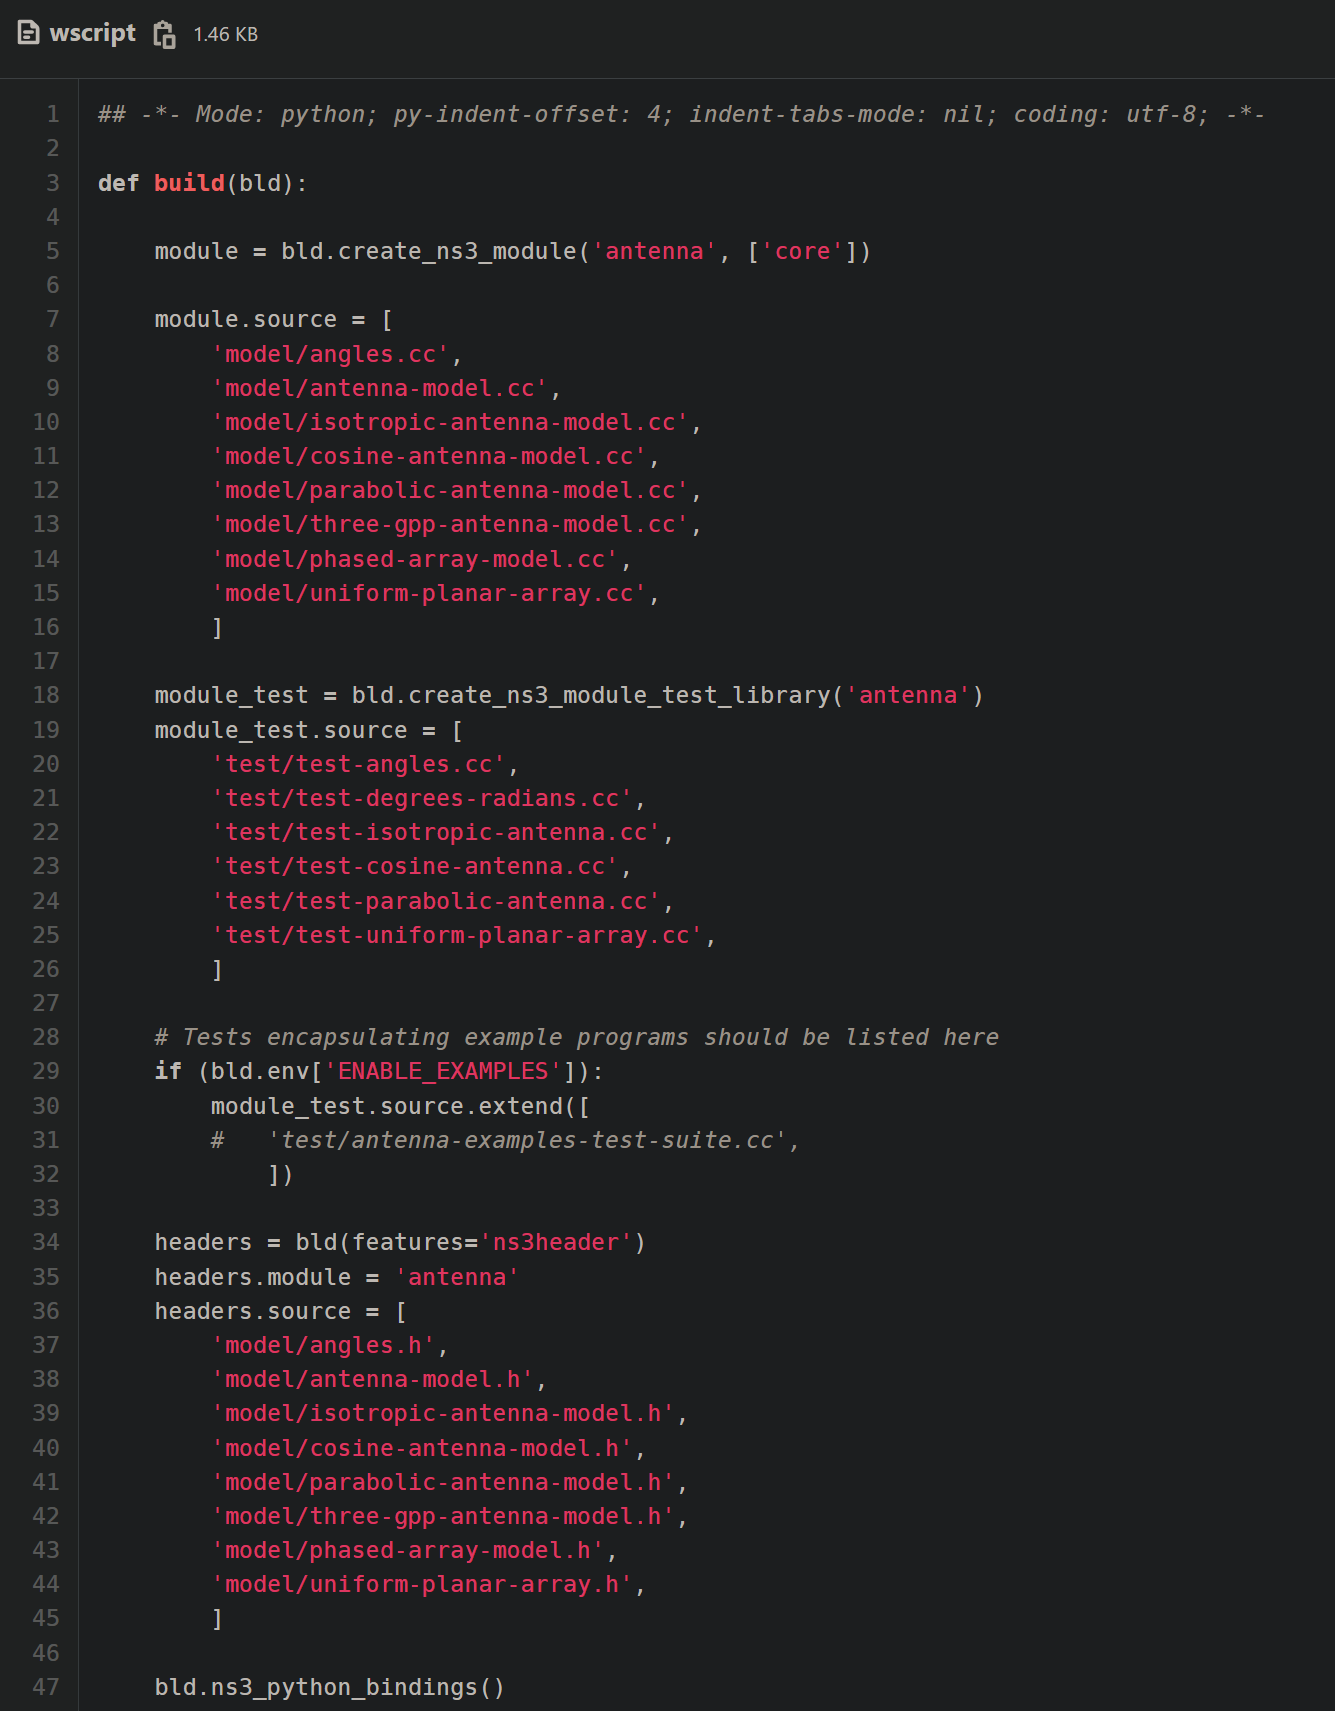
\includegraphics[width=0.45\linewidth]{antena_wscript.PNG} 
    \end{figure}
    
    \begin{figure}[h]
        \vspace{-15em}
        \hspace{+8em}
        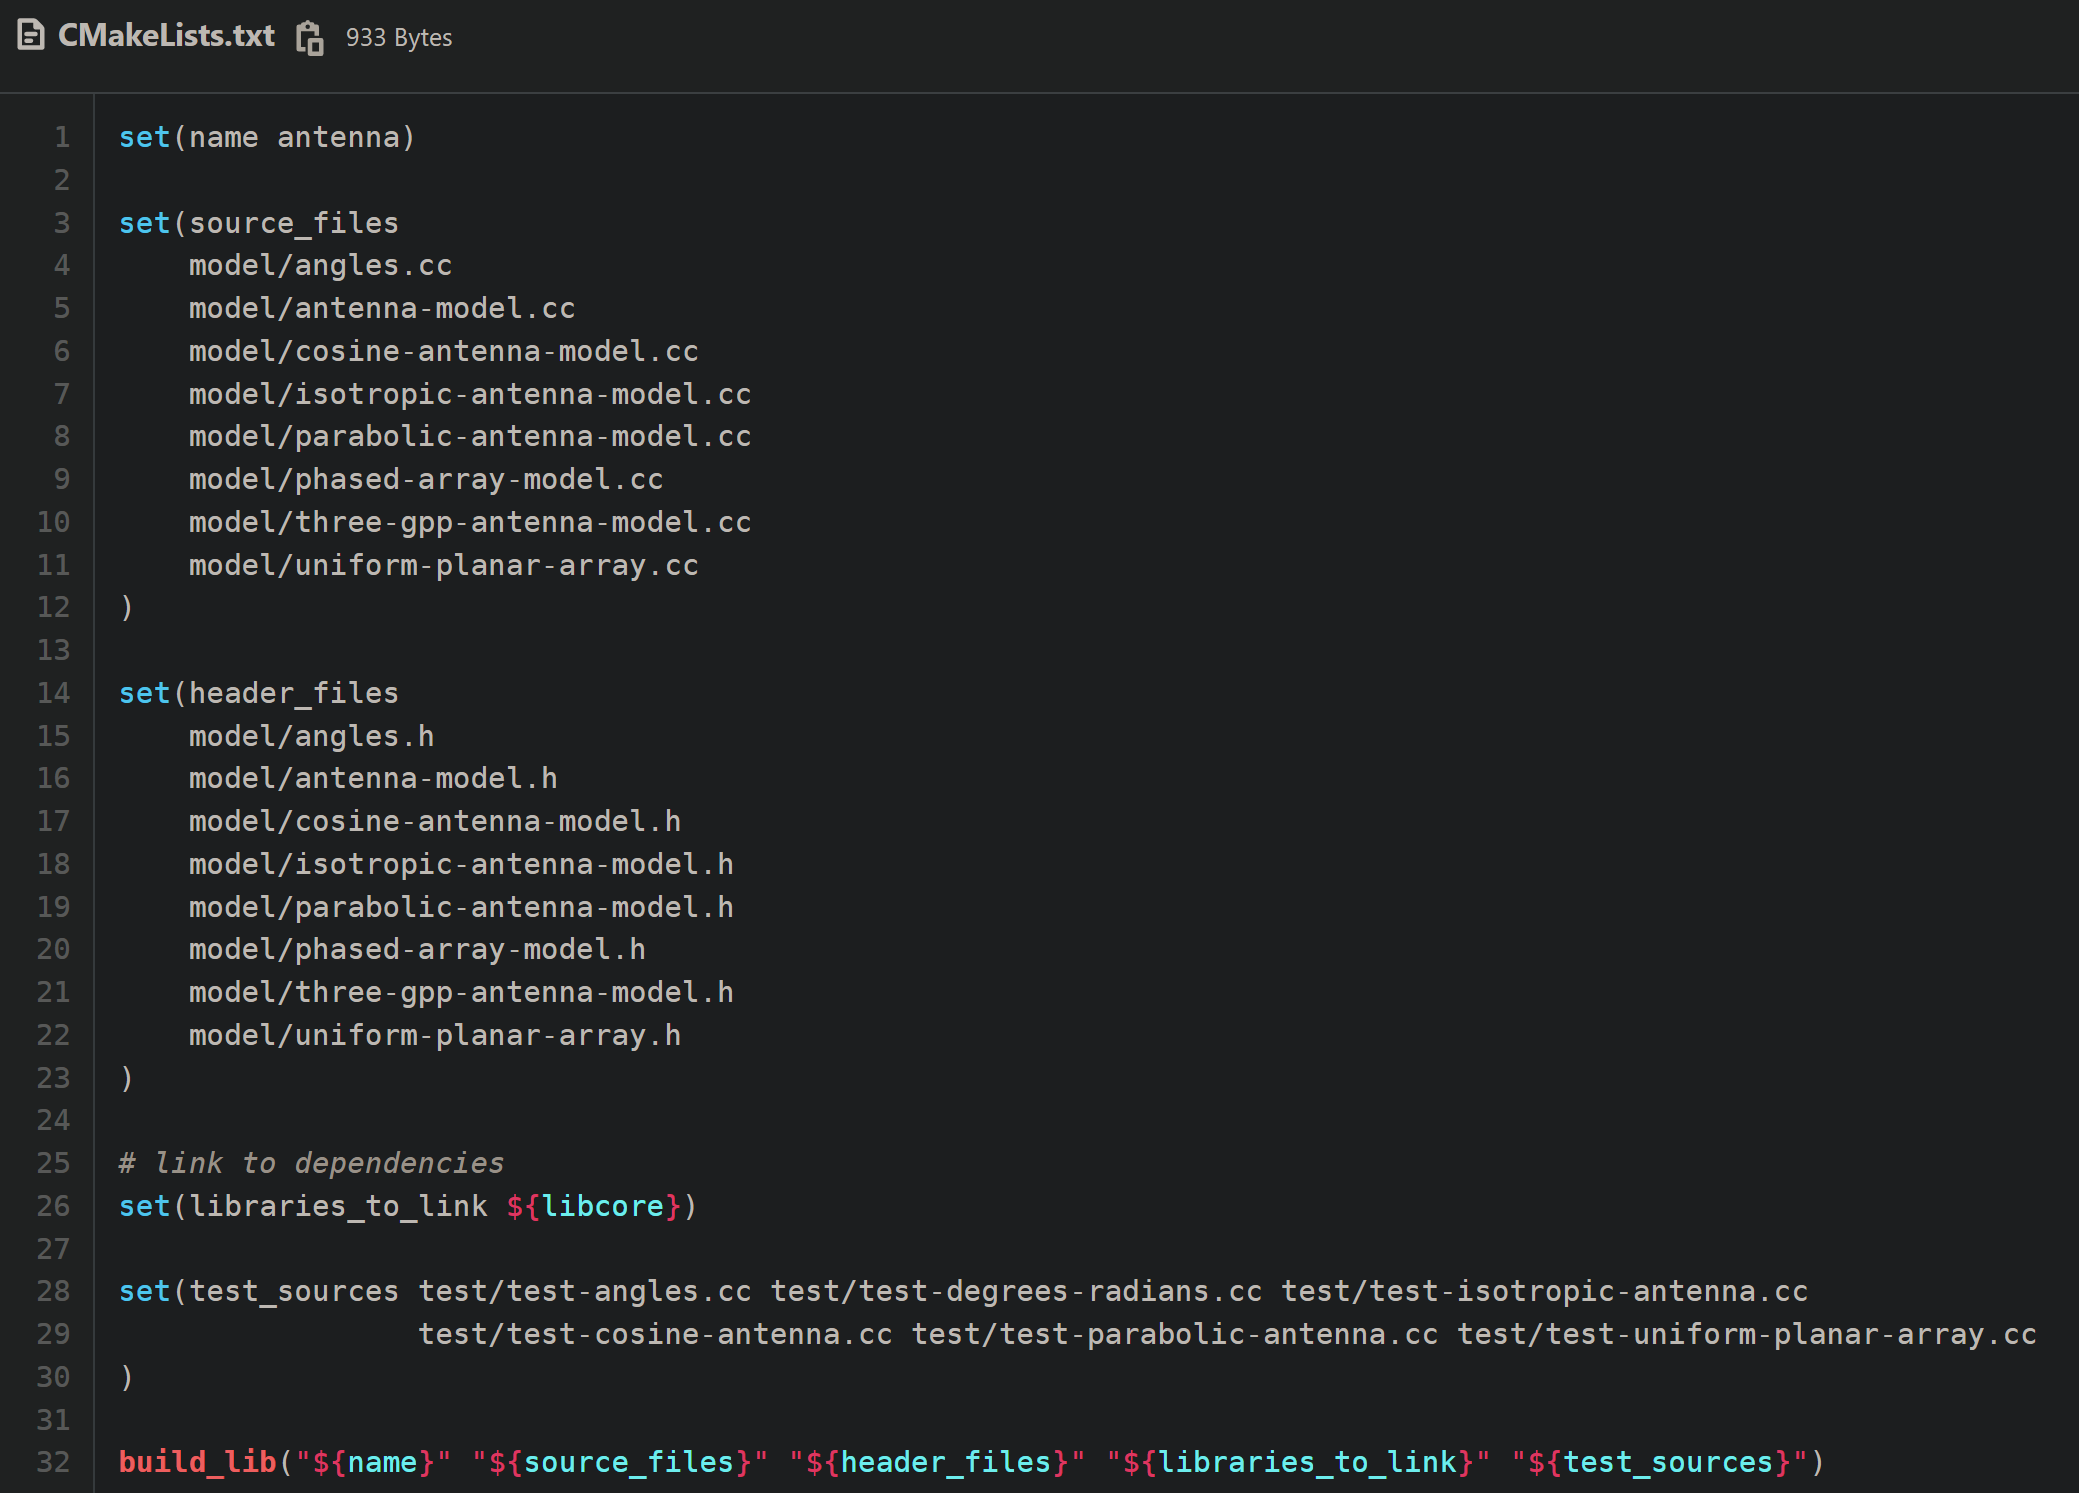
\includegraphics[width=0.45\linewidth]{antena_cmake.PNG}
    \end{figure}
\end{frame}

\begin{frame}{Current workflow}{Configure CMake}
    \begin{enumerate}
        \item This is required every time the CMake is changed
        \item[] \hspace{1em} {\footnotesize e.g. to include new source files or settings were changed}
        \item Previous options are preserved in the CMake cache
        \item[] \hspace{1em} {\footnotesize a.k.a. no need to pass all the options again when reconfiguring}
        \item Can be done either manually via terminal or GUI, or automatically via a config file (setting the flag values)
        \item[] {\footnotesize e.g. cmake --DCMAKE\_BUILD\_TYPE=debug --DNS3\_EXAMPLES=ON --DNS3\_TESTS=ON -G Ninja ..}
    \end{enumerate}
\end{frame}  

\begin{frame}{Current workflow}{Call the generated build system to build}
    \begin{enumerate}
        \item Call generated build system to build everything (or a specific target and its dependencies)
        \item[] {\footnotesize e.g. ninja (target)}

        
    \end{enumerate}
\end{frame}  

\begin{frame}{Current workflow}{Call binaries directly or via the IDE}
    \begin{enumerate}
        \item Works nicely on platforms that support RPATH, which is enabled by default (e.g. Linux and MacOS)
        \item Windows requires ns-3-dev/build in the PATH, which can be done automatically
        \item Something like waf --run, --gdb, --valgrind, --command-template, --pyrun, --visualize would require a wrapper script
    \end{enumerate}
\end{frame}  

\begin{frame}{Current workflow}{Debugging via the IDE: CLion}
    \begin{figure}[h]
        \vspace{-2em}
        \hspace{-2em}
        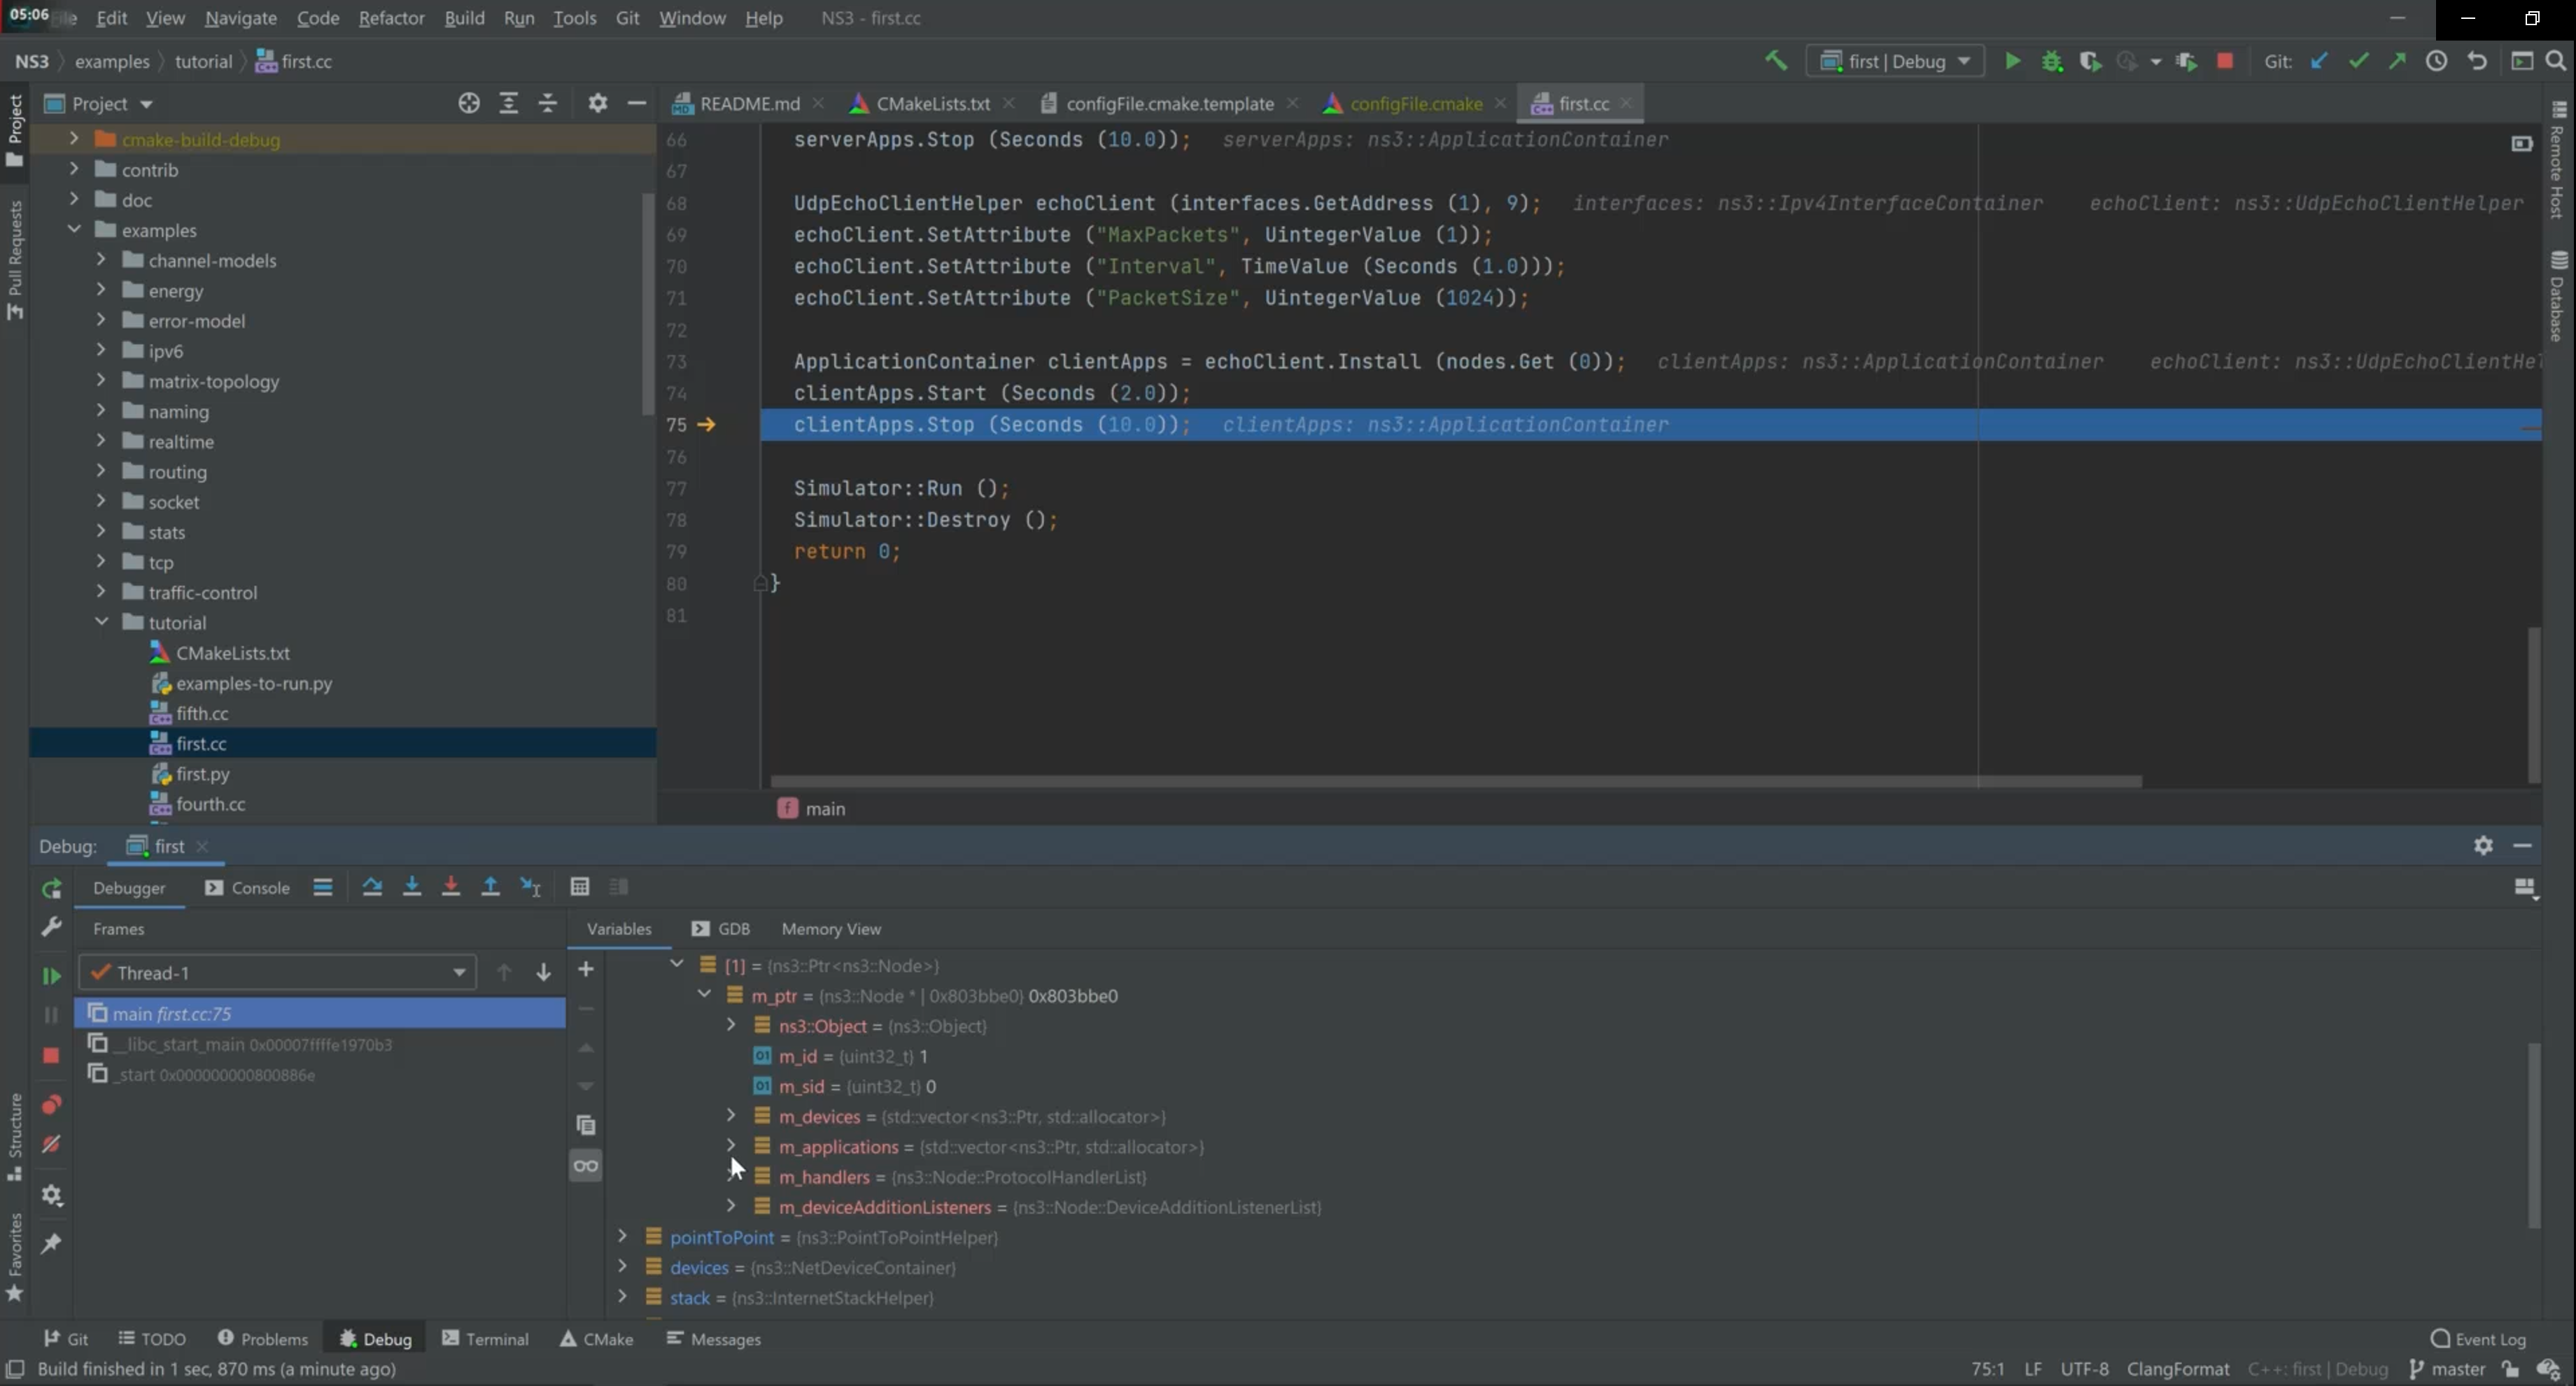
\includegraphics[width=0.9\linewidth]{debug_clion.png}
    \end{figure}
\end{frame} 

\begin{frame}{Current workflow}{Debugging via the IDE: Code::Blocks}
    \begin{figure}[h]
        \vspace{-2em}
        \hspace{-2em}
        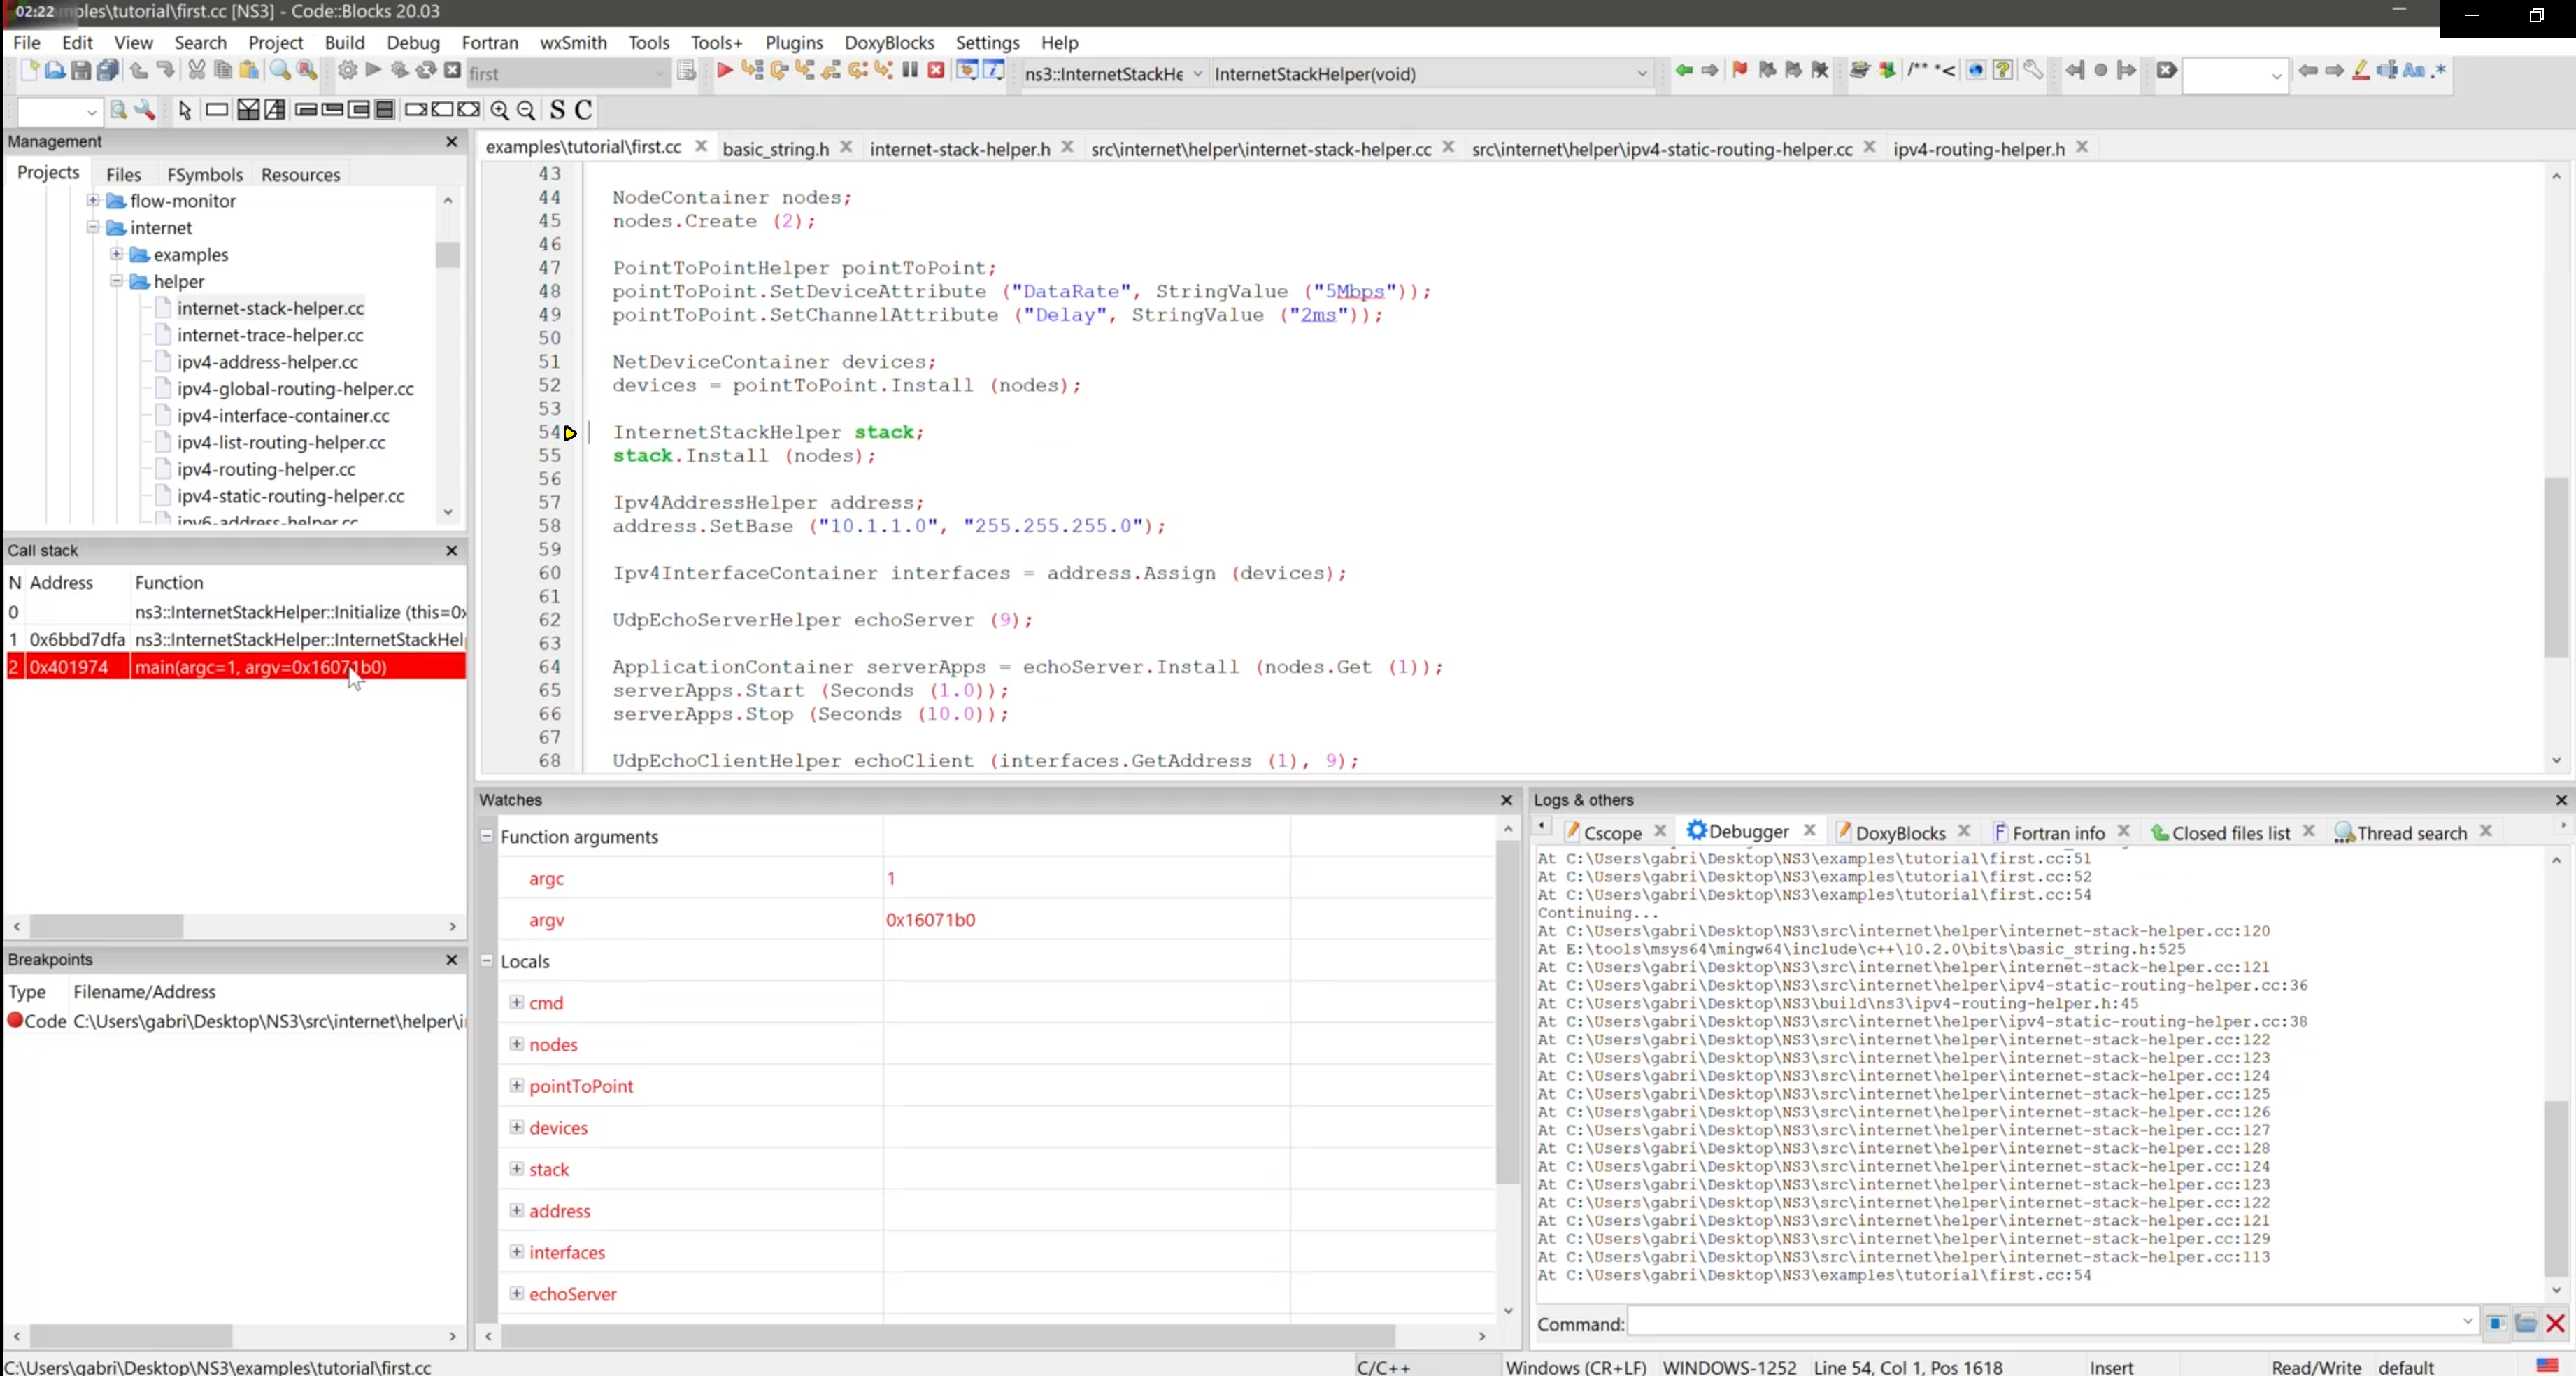
\includegraphics[width=0.9\linewidth]{debug_codeblocks.png}
    \end{figure}
\end{frame}  

\begin{frame}{Current workflow}{Debugging via the IDE: XCode}
    \begin{figure}[h]
        \hspace{-3em}
        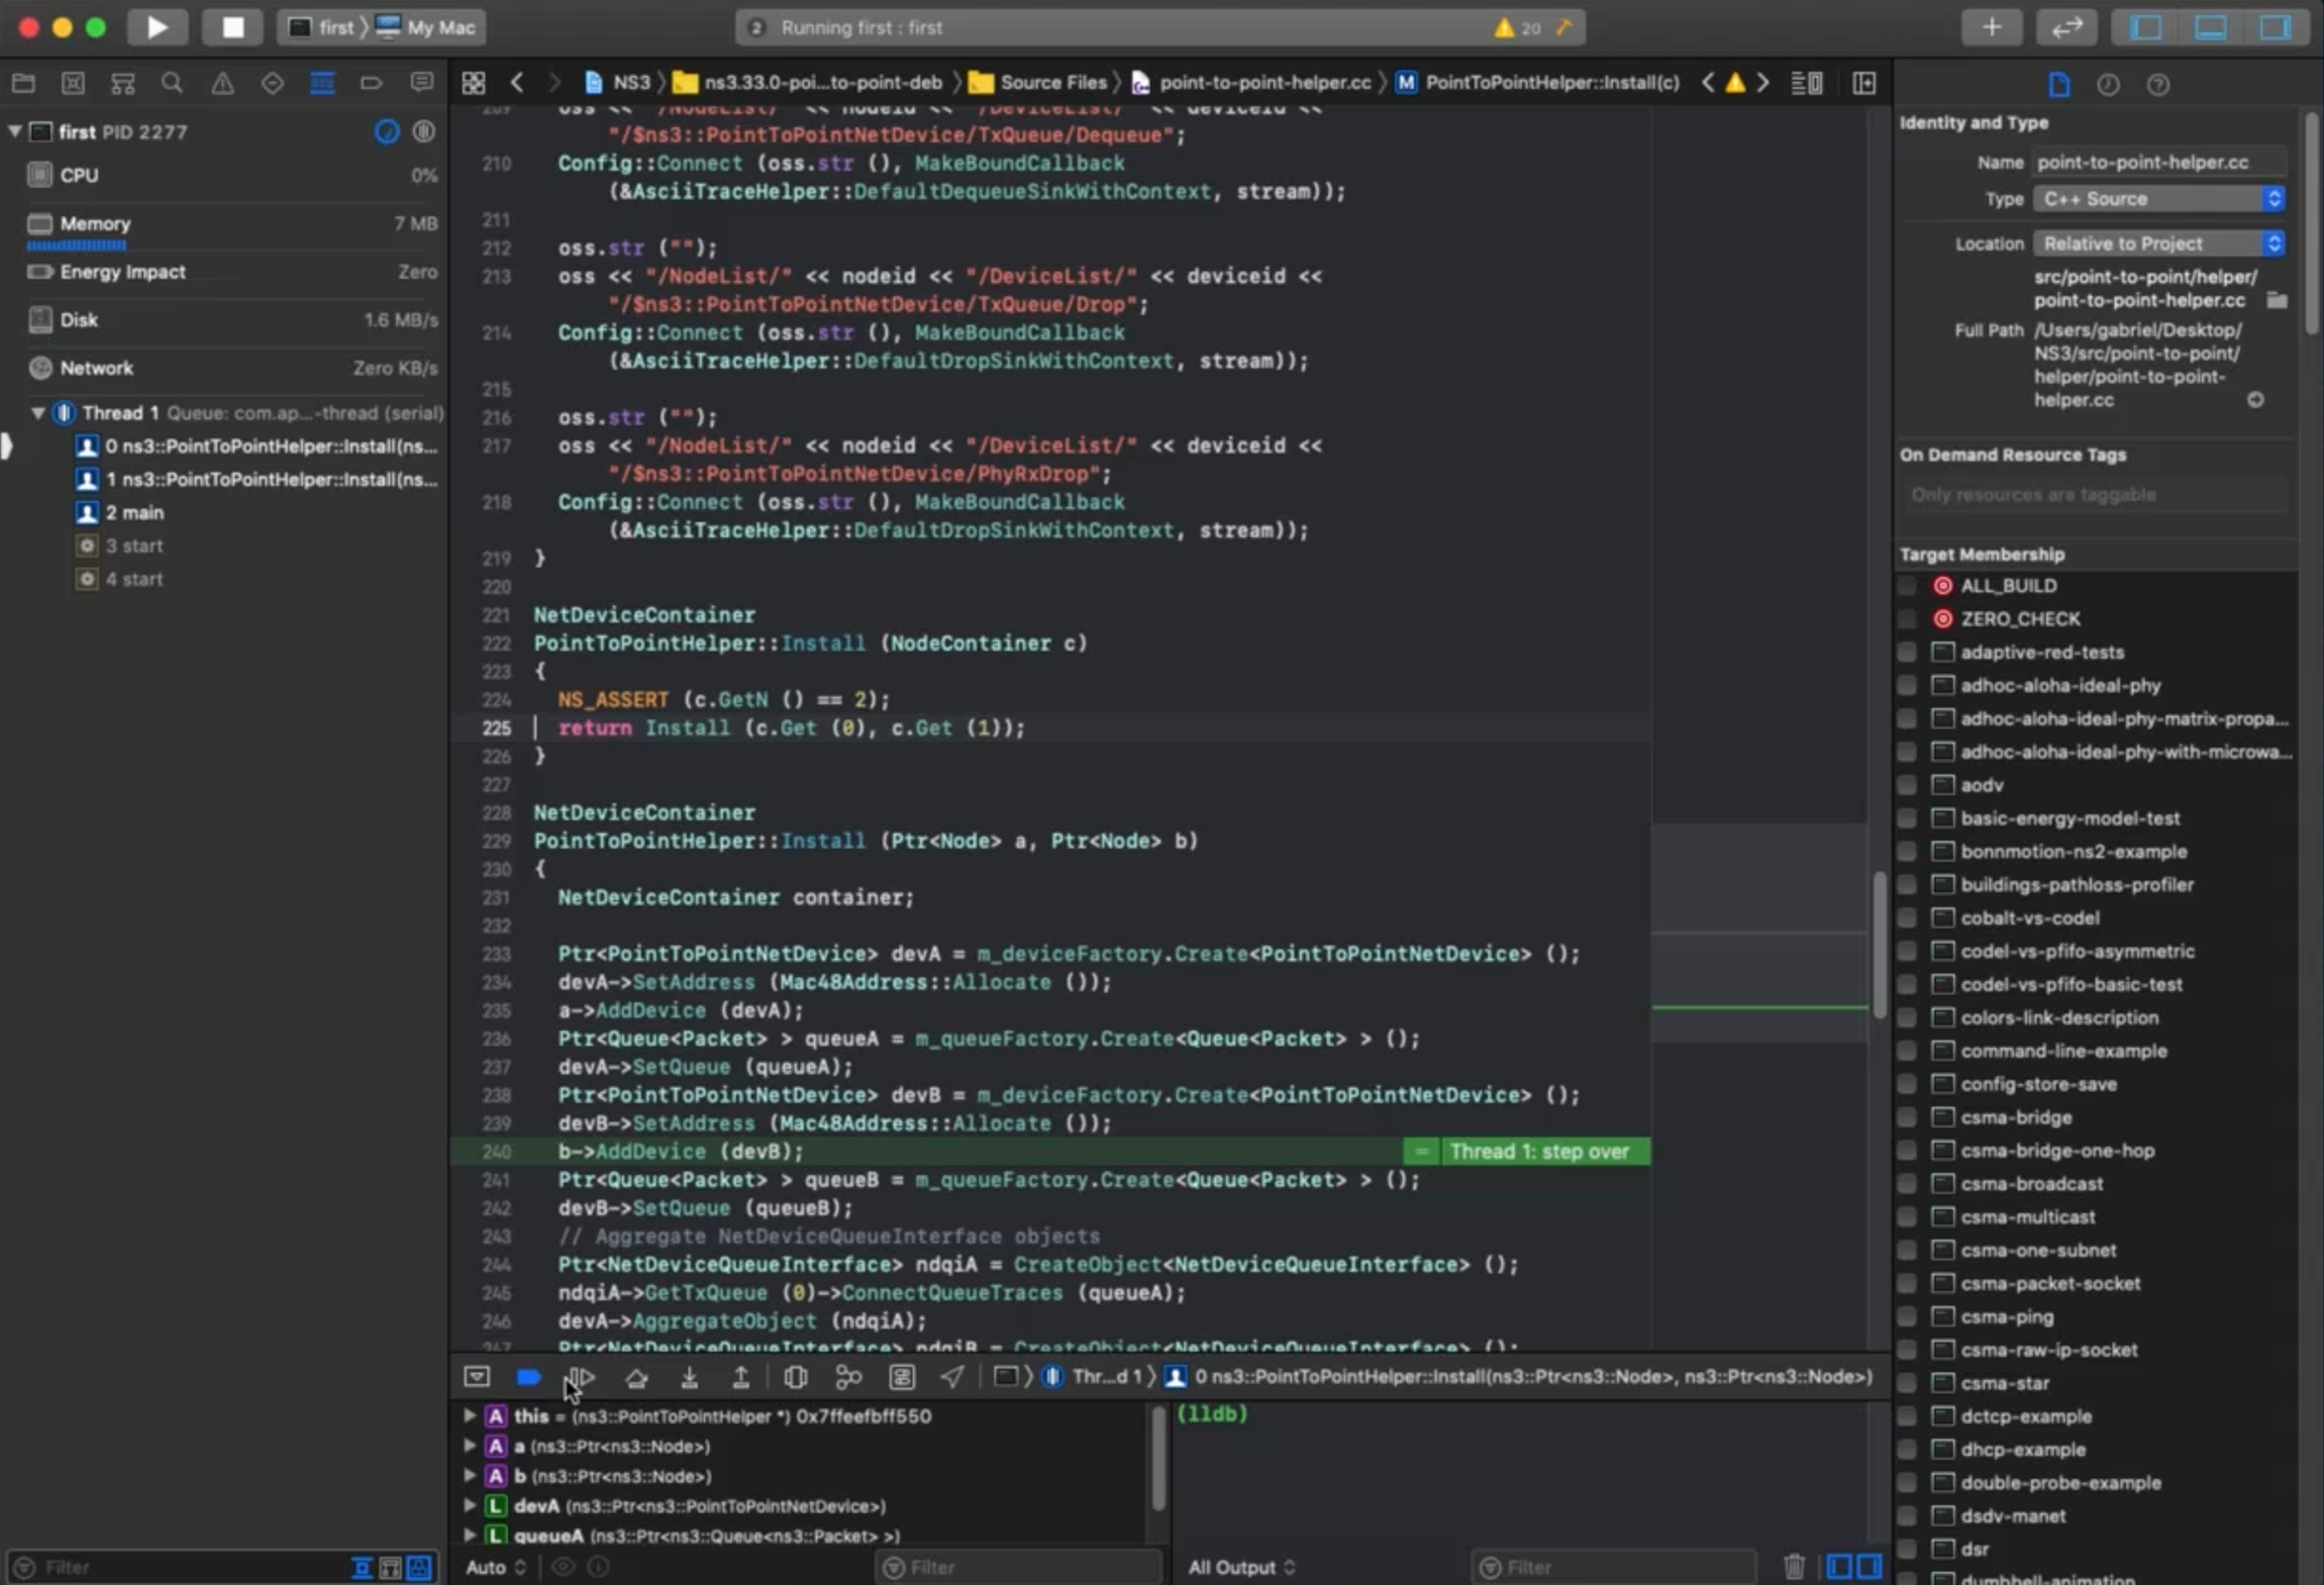
\includegraphics[width=0.95\linewidth]{debug_xcode.png}
    \end{figure}
\end{frame}  

\begin{frame}{Where is the code and instructions?}
    The instructions are in the MR 460:
    
    {\footnotesize https://gitlab.com/nsnam/ns-3-dev/-/merge\_requests/460}

    \vspace{1em}
    The sources are in the branch for the MR 460:
    
    {\footnotesize https://gitlab.com/Gabrielcarvfer/ns-3-dev/-/tree/buildsystem-cmake}
    
    \vspace{1em}
\end{frame} 

\begin{frame}{Questions? Concerns?}
    \centering
    You can find me on Zulip or via the email gabrielcarvfer@gmail.com

\end{frame}

\begin{frame}{}
    \centering Thank you for your time
    
\end{frame} 

\end{document}
